\documentclass[runningheads,a4paper]{llncs}

%\usepackage{bbding}%marvosymFor symbols of mail and tele
%\usepackage[utf8]{inputenc}
%\usepackage{fullpage}
\usepackage{amssymb}
\setcounter{tocdepth}{3}
\usepackage[pdftex]{graphicx}
%\usepackage{url}
%\usepackage[a4paper,margin=0in]{geometry}
%\usepackage[pdftex]{graphicx}
%\usepackage{anysize}
%\usepackage{times,tabularx,pifont}
%\usepackage{ae}
%\usepackage[T1]{fontenc}
%\usepackage{setspace}
\usepackage[hidelinks]{hyperref}
%\usepackage{research_paper}
%\usepackage{etoolbox}
%\usepackage{tikz}
\usepackage{enumerate}
\usepackage{multicol}
\setlength{\columnsep}{2cm}
\usepackage{url}
\urldef{\mailsa}\path|{hbhatt2014}@my.fit.edu|
\newcommand{\keywords}[1]{\par\addvspace\baselineskip
\noindent\keywordname\enspace\ignorespaces#1}
%\usepackage{enumitem}

%\usetikzlibrary{positioning,fit,patterns}

%\newlist{SubItem}{1}
%\setlist[SubItem]{label={$-$}}

%\renewcommand{\thesubitem}{\Roman{subitem}}

%\patchcmd{\thebibliography}{\section*{\refname}}{}{}{}

%\patchcmd{\thebibliography}{\addcontentsline{toc}{section}{\refname}}{}{}{}
%\usepackage[automark, headsepline, footsepline, plainheadsepline, plainfootsepline]{scrpage2}

%\setlength{\textwidth}{ 6in }
%\setlength{\textheight}{ 9.5in }

\renewcommand{\baselinestretch}{1.2}

%\renewcommand{\headrulewidth}{0pt}

%\newgeometry{[left=0.1in,right=0.2in,top=0.9in,bottom=0in]}

\begin{document}
%\marginsize{2in}{1in}{1in}{1in}
%\pagestyle{empty}

%\newgeometry{[left=0in,right=0.5in,top=1in,bottom=0in]}
\mainmatter

\title{Social World Connectivity among the Indian Celebrities}
\titlerunning{Social World Connectivity among the Indian Celebrities}

\author{Harshit Bhatt}
\authorrunning{Social World Connectivity among the Indian Celebrities}

\institute{Florida Institute of Technology, Melbourne - 32901\\
Florida, USA\\
\mailsa\\
\url{http://www.fit.edu/~hbhatt2014}} 

%\toctitle{Social World Connectivity among the Indian Celebrities}
%\tocauthor{Harshit Bhatt}
\maketitle

%\centerline{\fontsize{14}{18}{\textit{Research Paper on Twitter Data Mapping Project}}}
%\vspace{0.08in}
%\centerline{\fontsize{14}{18}{\textit{Complex Networks (CSE 5656)}}}
%\vspace{0.08in}
%\centerline{\fontsize{14}{18}{\textit{Fall 2014}}}

\begin{abstract}
This work maps social world(twitter) relationship among the Indian celebrities and groups based on their mention in tweets. Deducting the data helps in redefining the inter network of the celebrities and gave out various facts regarding users(tweeters) affiliation to the celebrities. The whole project helped me to gauge a new perspective of the Indian Celebrities in the social media which has not been thought about deeply in the past researches. This work not only explains the celebrities affiliations to general public but also their mindset.

%\par{Nodes in the network are various celebrities whereas the link (edges) between them is the common users. The link strength is measured by the number of common entities between nodes whereas the Node size is the number of unique user mentions for each celebrity. 
%Another network which forms a relationship among the celebrities on the basis of their mention in same tweets is made which helps to gauge the cohesiveness among the celebrities.}
%\paragraph{}
 %The networks gave some stark information about the celebrities, as we saw in different networks the major player(according betweenness centrality) were different due to the different factors on which the respective network was developed. The networks could be said biased due to various events concerning specific celebrities during tweet collection time which spiked the mention of those celebrities and their relationship.
%
%\paragraph{}
 %- about what they are more likely to tweet about and if done further research on the semantics of the tweets it could lead in defining personal relationships between specific tweeters and celebrities.

\keywords{Twitter API, Social Media, Relationship between Users and Celebrities}
\end{abstract}

\section{Introduction}

\paragraph{}
The main purpose of devising this network was to get a gauge of the celebrities fame and their inter-network through the Social Media Data. The data here is the tweets, and only those tweets are included which mention or are related to, any of these Celebrities or groups. Only those celebrities and groups are included who are verified from Twitter.

\paragraph{}Celebrities in the list are from the field of Indian Cinema, Cricket and Politics. Due to the popularity of the celebrities among their fan base I was able to collect a large amount of data with the help of Twitter Streaming API.

\paragraph{}
The JSON data given by Twitter API includes a wide range of information about a tweet, which helped in defining the base table for the network, through which I was able to deduce various other meaningful sub-tables and views which modeled the various graphs in my result.

\paragraph{}
Tables which mapped the various graphs were on :

\begin{itemize}

\item List of number of unique users for each celebrity

\item List of common users between each pair of celebrities

\item List of total number of each celebrity mentioned in tweets

\item List of each pair of celebrities who are mentioned in the same tweet and their count

\item List of every user and their mention counts to the celebrity(this list is for each celebrity)

\item List containing hashtags related to celebrities

\item List having common hashtags reference between the celebrities

\end{itemize}

\paragraph{}
There were three networks that were constructed with these tables and their result has been shown in the Result section of this report. The networks had a lot of edges between them which I reduced with the filters in Gephi to get a common overview of the network so only the most prominent nodes were left in the network. The nodes size was taken in accordance to their betweenness centrality which gives a more real clout of the celebrities in the network, the edge strength is similar as initially thought of - the number of relations between the celebrities more thick edge means more celebrities are related to each other. The network structure is developed through OpenOrd layout of Gephi with node color in accordance to the modularity class and community division also done with help of it.

\paragraph{}
With help of Gephi I was able to calculate degree distribution, betweenness and closeness centrality, eccentricity, density and modularity of the network whose result I have shown in the Result section for further detailed study of the networks.

%\par { The first two tables make a network which proposes the common interest among users between celebrities, in this network : }
%
%\vspace{0.1in}
%
%\centerline { Nodes -$>$ Celebrities } 
%\centerline { Node Size -$>$ Celebrities unique users count } 
%\centerline { Edges -$>$ Common Users between celebrities } 
%\centerline { Edge Strength -$>$ Common Users count }
%
%\vspace{0.2in}
%
%\par { The third and fourth table define a network which proposes how commonly two celebrities are mentioned in the same tweets, in this network : }
%
%\vspace{0.1in}
%
%\centerline { Nodes -$>$ Celebrities } 
%\centerline { Node Size -$>$ Celebrities mention count } 
%\centerline { Edges -$>$ Celebrities common in a tweet } 
%\centerline { Edge Strength -$>$ Celebrities common in a tweet count }

\section{Building the Twitter Network}

\begin{itemize}

\item The first step was to set up Twitter Streaming API which was processed by getting my special token and secret key from twitter for this application.

\item The python library Tweepy was used as a bridge to collect tweets from the Twitter Inc.

\item The whole program is set up in the Python language, which helped to collect tweets and its other relevant information, which was further saved into MySQL database tables so as to map the networks.

\item The main table for the network is named celebrity\_tweets which includes the first data that is collected directly from the tweets.

\item The fields are -$>$

\subitem	user\_twitter\_id  -$>$  it has the twitter id of the person who has send that tweet.
\subitem	user\_name  -$>$  user twitter handle.
\subitem	tweet  -$>$  the actual tweet which has been sent by the user.
\subitem	users\_mention\_id  -$>$  twitter id of the celebrities that are mentioned in the tweet.
\subitem	hashtags -$>$ hashtags that are in the tweet and are related to those celebrities. 

\item	To get all (most of) the celebrities in India I first choose three most famous Indian celebrities(based on general prospective) which by their twitter handle are @SrBachchan, @iamsrk, @msdhoni. 

\item	With the help of Twitter API I was able to collect all the Verified friends and friends of friends of these celebrities.

\item	Each of these friends details are saved by their respective table name having fields as :

\subitem	user\_id  -$>$  celebrity twiiter id
\subitem	user\_name -$>$ celebrity twitter handle

\item	The same was done for the first three celebrities for their friends list and their own details.

\item	Now a list was made to remove the duplicates from these tables and get a unique list of celebrities which was saved in the table named celebrities.

\item This list was saved to a table named celebrities which holds detail for every celebrity used in our tweet collection. It has fields as :

\subitem	celebrity\_twitter\_id  -$>$  celebrity twiiter id
\subitem	celebrity\_twitter\_name -$>$ celebrity twitter handle

\item	There were total of 467 unique celebrities and verified groups which I finally got as the input for data collection.

\item	The program is now executed with the input of these unique celebrities.

\item	The data collected is saved in the celebrity\_tweets table as discussed above.

\item	The data was collected within a range of 23 days and total tweets collected were around 352,000.

\item	After the data collection some relevant tables were deduced from the main table, which were respectively related to the specific networks which we have mapped to show the final results.
\vspace{0.1in}
\item Those were Six tables namely : 
\vspace{0.1in}
\subitem	a. celebrity\_mentions\_count -$>$ this table stores the total mentions which a celebrity received during the time period. It has fields as : 

\begin{enumerate}[i.  ]
\addtolength{\itemindent}{1cm}
\item celebrity\_twitter\_id -$>$ celebrity twitter id
\item nodes -$>$ celebrity twitter handle
\item weight -$>$ total user mentions
\end{enumerate}
\vspace{0.1in}
\subitem b. celebrity\_common\_mention\_tweets -$>$ this table gives the number of tweets in which the celebrities are commonly mentioned. It has fields as :

\begin{enumerate}[i.  ]
\addtolength{\itemindent}{1cm}
\item source -$>$ one of the celebrities twitter handle in the pair
\item celebrity1\_id -$>$ first celebrity twitter id
\item target -$>$ the other celebrity twitter handle in the pair
\item celebrity2\_id -$>$ second celebrity twitter id
\item weight -$>$ number of tweets having celebrities common mentioned
\end{enumerate}
\vspace{0.1in}
\subitem  c. celebrity\_specific\_distinct\_hashtags\_count -$>$ this table gives the total number of different hashtags that are connected to the celebrity. It has fields as :

\begin{enumerate}[i.  ]
\addtolength{\itemindent}{1cm}
\item celebrity\_twitter\_id -$>$ celebrity twitter id
\item nodes -$>$ celebrity twitter handle
\item weight -$>$ total distinct hashtags connected with the celebrity
\end{enumerate}
\vspace{0.1in}
\subitem d. celebrity\_hashtags\_common -$>$ this table gives the number of hashtags that are common between each pair of celebrities. It has fields as :

\begin{enumerate}[i.  ]
\addtolength{\itemindent}{1cm}
\item source -$>$ one of the celebrities twitter handle in the pair
\item celebrity1\_id -$>$ first celebrity twitter id
\item target -$>$ the other celebrity twitter handle in the pair
\item celebrity2\_id -$>$ second celebrity twitter id
\item weight -$>$ number of hashtags that are common between them
\end{enumerate}
\vspace{0.1in}
\subitem e. celebrity\_number\_unique\_users -$>$ this table gives the total unique users that a celebrity got mentioned by. It has fields as :

\begin{enumerate}[i.  ]
\addtolength{\itemindent}{1cm}
\item celebrity\_twitter\_id -$>$ celebrity twitter id
\item nodes -$>$ celebrity twitter handle
\item weight -$>$ number of unique users for the celebrity
\end{enumerate}
\vspace{0.1in}
\subitem f. celebrity\_users\_common -$>$ this table gives the number of users that are common between each pair of celebrities. It has fields as :

\begin{enumerate}[i.  ]
\addtolength{\itemindent}{1cm}
\item source -$>$ one of the celebrities twitter handle in the pair
\item celebrity1\_id -$>$ first celebrity twitter id
\item target -$>$ the other celebrity twitter handle in the pair
\item celebrity2\_id -$>$ second celebrity twitter id
\item weight -$>$ number of users that are common between them
\end{enumerate}

\item	I have also saved the users details who have mentioned the celebrity in another database with tables name respective of the celebrity name containing the fields as : 
  
\subitem user\_id -$>$ user twitter id who has mentioned that celebrity
\subitem user\_name -$>$ users twitter handle
\subitem count -$>$ number of times that celebrity has been mentioned by the user

\item	Three networks were constructed with the help of the above six tables. With help of igraph python library and Gephi Software we were able to map these networks. The networks are as following : 
\vspace{0.1in}
\subitem	a. The first network uses celebrity\_users\_common and celebrity\_number\_unique\_users tables to generate a relationship which proposes the common users between each pair of celebrities, in this network :
\vspace{0.1in}
\begin{enumerate}[i.  ]
\addtolength{\itemindent}{1cm}
\item Nodes -$>$ Celebrities
\item Node Size -$>$ Celebrities unique users count
\item Edges -$>$ Common Users between Celebrities
\item Edge Strength -$>$ Common Users count
\end{enumerate}
\addtolength{\itemindent}{-0.5cm}
\vspace{0.1in}
\textbf{For example =$>$}
\begin{flushleft}
\centerline{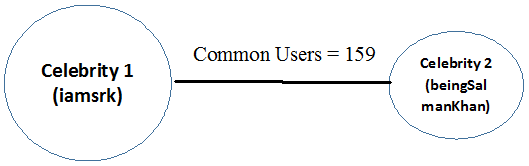
\includegraphics[width=0.7\textwidth,height=0.5\textheight,keepaspectratio]{common_users_eg_1.png}}
\centerline{Unique Users = 6353 \hspace{2cm} Unique Users = 852}
\vspace{0.2in}
\centerline{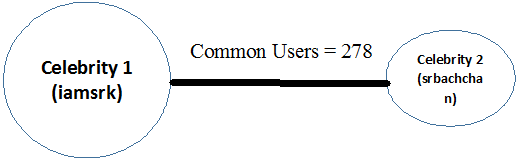
\includegraphics[width=0.7\textwidth,height=0.5\textheight,keepaspectratio]{common_users_eg_2.png}}
\centerline{Unique Users = 6353 \hspace{2cm} Unique Users = 797}
\end{flushleft}
\subitem b. The second network uses celebrity\_mentions\_count and celebrity\_common\_mention\_tweets tables to generate a relationship which proposes how commonly two celebrities are mentioned in the same tweets, in this network :
\vspace{0.1in}
\begin{enumerate}[i.  ]
\addtolength{\itemindent}{1cm}
\item Nodes -$>$ Celebrities
\item Node Size -$>$ Celebrities mention count
\item Edges -$>$ Celebrities common in a tweet
\item Edge Strength -$>$ Celebrities count commonly mentioned in tweet
\end{enumerate}
\vspace{0.1in}
\textbf{For example =$>$}
\begin{flushleft}
\centerline{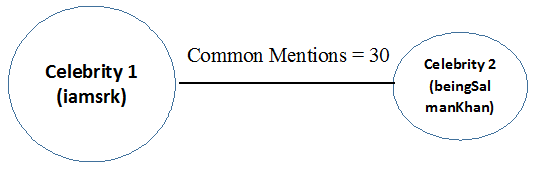
\includegraphics[width=0.7\textwidth,height=0.5\textheight,keepaspectratio]{common_mention_eg_1.png}}
\centerline{Total Mentions = 23443 \hspace{2cm} Total Mentions = 1693}
\vspace{0.2in}
\centerline{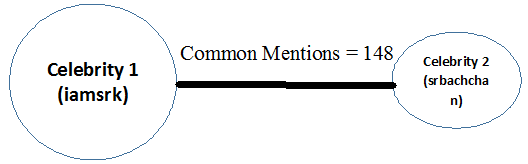
\includegraphics[width=0.7\textwidth,height=0.5\textheight,keepaspectratio]{common_mention_eg_2.png}}
\centerline{Total Mentions = 23443 \hspace{2cm} Total Mentions = 1087}
\end{flushleft}
\subitem c. The third network uses celebrity\_specific\_distinct\_hashtags\_count and celebrity\_hashtags\_common tables to generate a relationship which proposes how many hashtags are common between the celebrities, in this network :
\vspace{0.1in}
\begin{enumerate}[i.  ]
\addtolength{\itemindent}{1cm}
\item Nodes -$>$ Celebrities
\item Node Size -$>$ Celebrities hashtags count
\item Edges -$>$ Celebrities common hashtags
\item Edge Strength -$>$ count of Celebrities common hashtags
\end{enumerate}
\vspace{0.1in}
\textbf{For example =$>$}
\begin{flushleft}
\centerline{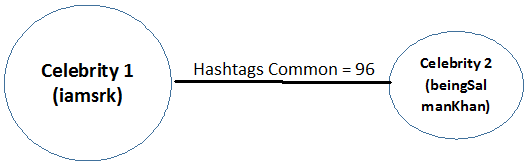
\includegraphics[width=0.7\textwidth,height=0.5\textheight,keepaspectratio]{common_hashtags_eg_1.png}}
\centerline{Total Mentions = 1165 \hspace{2cm} Total Mentions = 276}
\vspace{0.2in}
\centerline{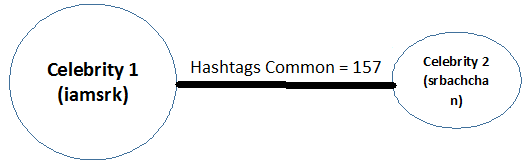
\includegraphics[width=0.7\textwidth,height=0.5\textheight,keepaspectratio]{common_hashtags_eg_2.png}}
\centerline{Total Mentions = 1165 \hspace{2cm} Total Mentions = 376}
\end{flushleft}
\end{itemize}

\section{Related Work}

\paragraph{}
Many such networks regarding the relationships among celebrities have been developed in the past by researchers. As the celebrities hold a special status in general public mind and hence their demeanor, their words affect people a lot which has made researchers to work on this field with extreme enthusiasm. We here would be talking about three main research which made me to opt for this topic.
\paragraph{}
Most of the research in this field is based on the public database of IMDB which include every actor and their movies and where they have worked with each other and hence a relationship could be formed.
\paragraph{}
There has been no such research on Indian celebrities social media relationship in the past which made me to delve into this field. My main inspiration comes from a surprising source - a blog which I read while surfing on the internet of Fafadia Tech \cite{fafadia} where they have shown a relationship between the Indian actors on the context of those celebrities working together, the data for which they got from the IMDB databse but I tried to extend that work by taking Social Media in the context and using real world common public tweets for drawing a relation between these celebrities which could show a more genuine relationship between the Indian celebrities.
\paragraph{}
Some other work related to the affiliation between the Movies and Actors in the Hollywood was conducted by researchers \cite{1} where they conducted the same experiment as above for the actors and their affiliation with the movies they have worked on using the IMDB database.
\paragraph{}
Another work related on the analysis and measurement of social network \cite{2} also helped me to finalize the basic theme and initial setup of my network where researchers have shown how does the social network would be used as a genuine medium of measuring various real world entities in the near future as more people are concentrating on this medium for communicating and expressing their thoughts and ideas.

\section{Experimental Results}

\centerline{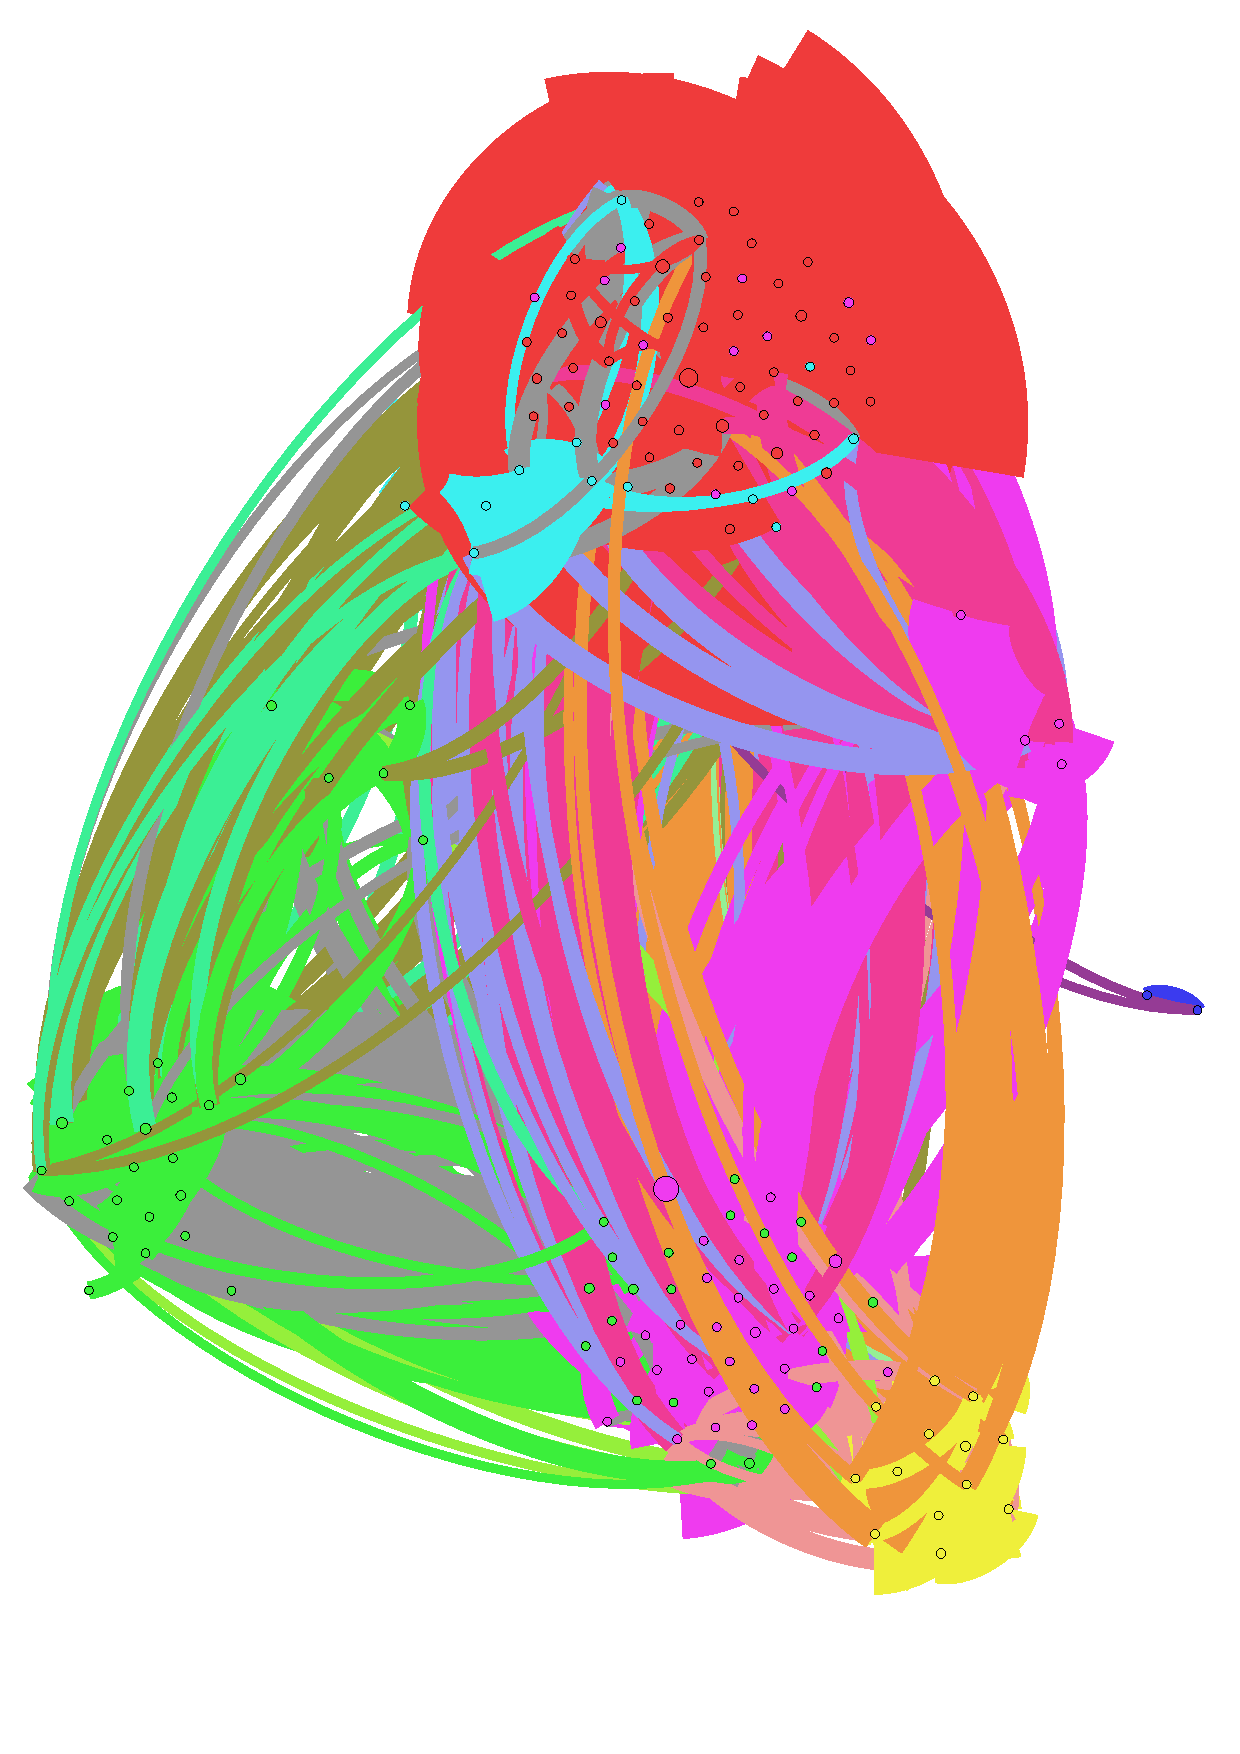
\includegraphics[width=\textwidth,height=\textheight,keepaspectratio]{users_common_network.png}}
\vspace{0.1in}
\centerline{Common Users between Celebrities Community Network}
\vspace{0.2in}
\noindent{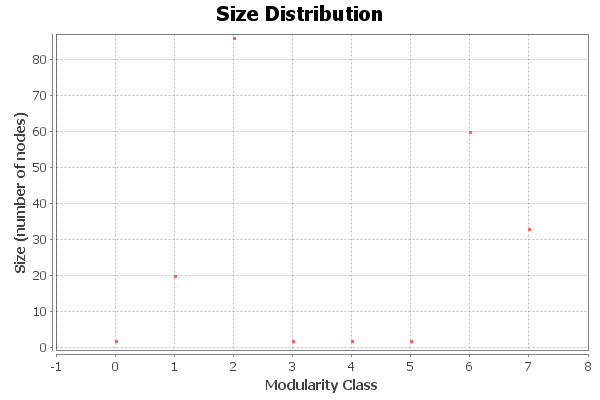
\includegraphics[width=0.45\textwidth,height=0.5\textheight,keepaspectratio]{users_common_modularity_graph.png}}\hspace{1.2cm}
\noindent{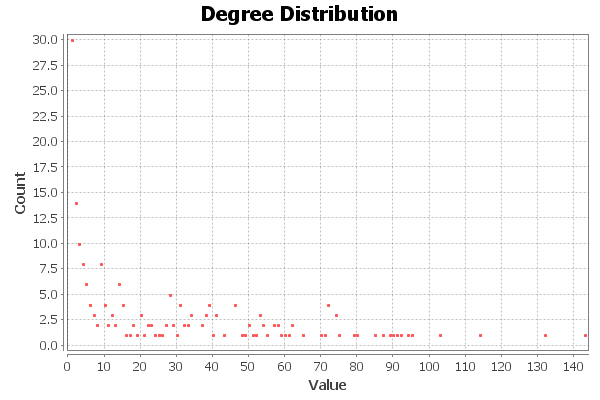
\includegraphics[width=0.45\textwidth,height=0.5\textheight,keepaspectratio]{users_common_degree_graph.png}}
\vspace{-0.5cm}
\begin{multicols}{2}{Graph for the Communities Distribution of Common Users Network}\vfill\columnbreak{Graph for the Degree Distribution of Common Users Network}\end{multicols}
\vspace{-0.5cm}
\begin{multicols}{2}{\noindent{\fontsize{10}{12}{\textbf{Results =$>$ Modularity: 0.351, Modularity with resolution: 0.280, Number of Communities: 8}}}}\vfill\columnbreak{\noindent{\fontsize{10}{12}{\textbf{Results =$>$ Average Degree: 26.947}}}}\end{multicols}
\vspace{-0.4cm}
\noindent{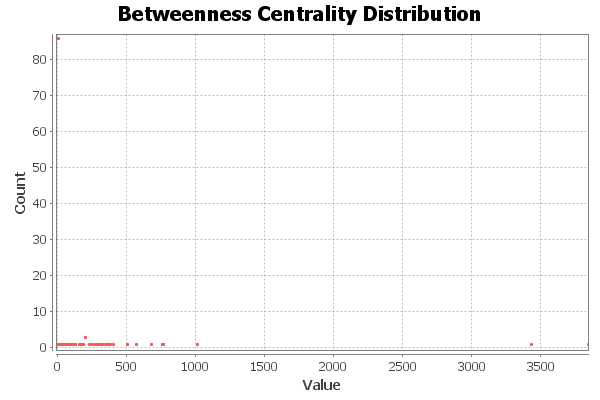
\includegraphics[width=0.45\textwidth,height=0.5\textheight,keepaspectratio]{users_common_betweenness_graph.png}}\hspace{1.2cm}
\noindent{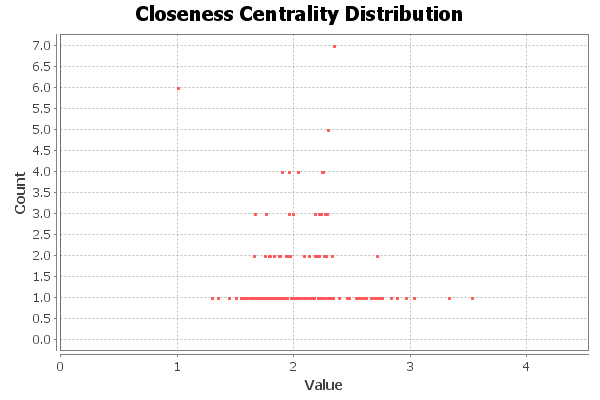
\includegraphics[width=0.45\textwidth,height=0.5\textheight,keepaspectratio]{users_common_closeness_graph.png}}
\vspace{-0.5cm}
\begin{multicols}{2}{\noindent{Graph for Betweenness Centrality Distribution of Common Users Network}}\vfill\columnbreak{\noindent{Graph for Closeness Centrality Distribution of Common Users Network}}\end{multicols}
\vspace{-0.2cm}
\centerline{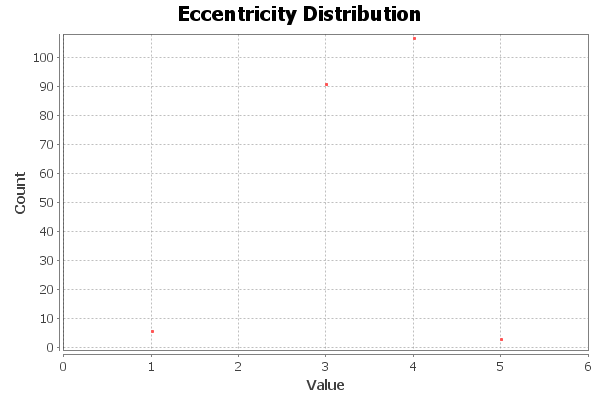
\includegraphics[width=0.5\textwidth,height=0.5\textheight,keepaspectratio]{users_common_eccentricity_graph.png}}
\centerline{Graph for Eccentricity Distribution of Common Users Network}
\vspace{0.2in}
\centerline{\fontsize{10}{12}{\textbf{Results =$>$ Diameter: 5, Radius: 1, Average Path length: 2.0907, Number of shortest paths: 40206}}}
\vspace{0.2in}
\centerline{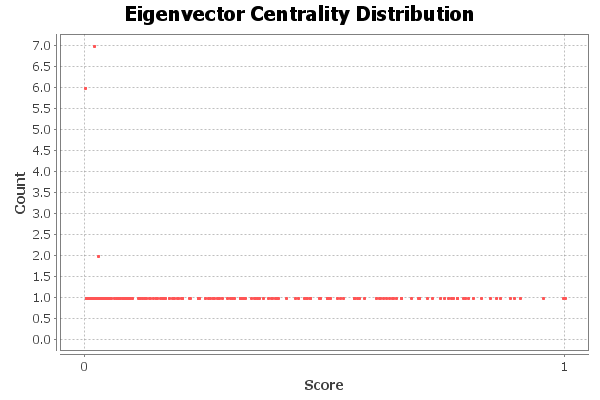
\includegraphics[width=0.5\textwidth,height=0.5\textheight,keepaspectratio]{users_common_eigenvector_graph.png}}
\centerline{Graph for EigenVector Centrality Distribution of Common Users Network}
\vspace{0.2in}
\centerline{\fontsize{10}{12}{\textbf{Parameters =$>$ Number of iterations: 100, Sum change: 0.006464}}}

\begin{figure}
\centering
\includegraphics[width=\textwidth,height=\textheight,keepaspectratio]{common_mention_network.png}
\caption{Celebrities mention in same tweet Community Network}
\end{figure}

\begin{figure}
\noindent{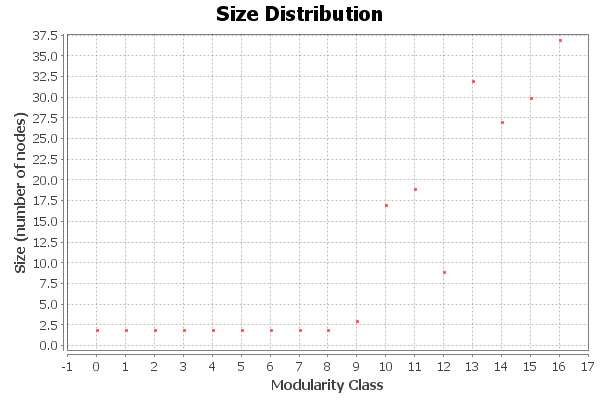
\includegraphics[width=0.45\textwidth,height=\textheight,keepaspectratio]{common_mention_modularity_graph.png}}\hspace{1.8cm}{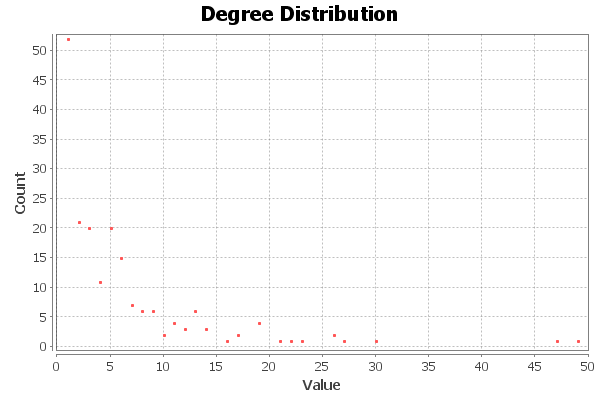
\includegraphics[width=0.45\textwidth,height=\textheight,keepaspectratio]{common_mention_degree_graph.png}}
\begin{multicols}{2}{\caption{Graph for the Communities Distribution of Common Mention Network}}\vfill\columnbreak{\caption{Graph for the Degree Distribution of Common Mention Network}}\end{multicols}
\begin{multicols}{2}{\noindent{\fontsize{10}{12}{\textbf{Results =$>$ Modularity: 0.580, Modularity with resolution: 0.495, Number of Communities: 17}}}}\vfill\columnbreak{\noindent{\fontsize{10}{12}{\textbf{Results =$>$ Average Degree: 6.021}}}}\end{multicols}
\end{figure}

\begin{figure}
\noindent{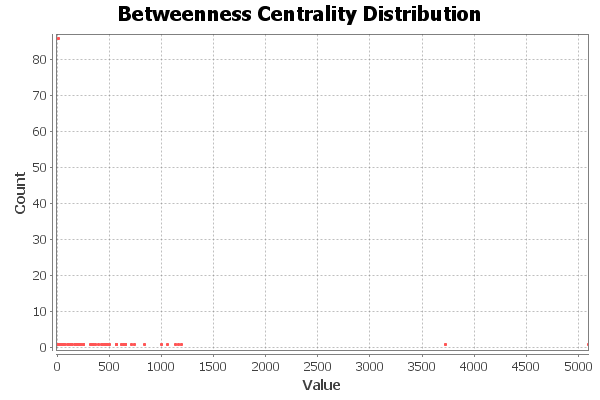
\includegraphics[width=0.45\textwidth,height=\textheight,keepaspectratio]{common_mention_betweenness_graph.png}}\hspace{1.8cm}{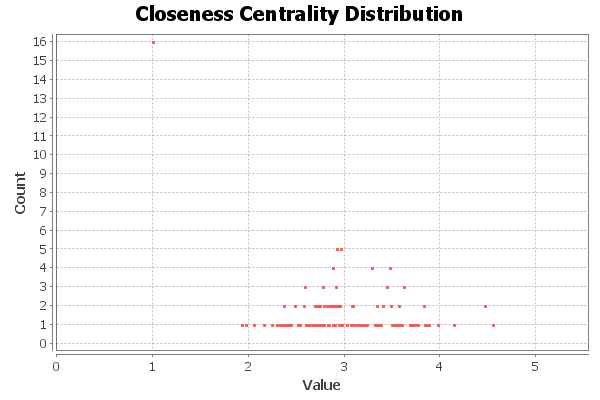
\includegraphics[width=0.45\textwidth,height=\textheight,keepaspectratio]{common_mention_closeness_graph.png}}
\begin{multicols}{2}{\caption{Graph for Betweenness Centrality Distribution of Common Mention Network}}\vfill\columnbreak{\caption{Graph for Closeness Centrality Distribution of Common Mention Network}}\end{multicols}
\end{figure}

\begin{figure}
\centerline{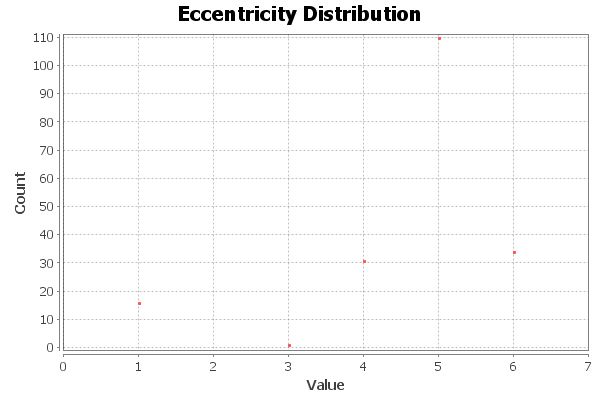
\includegraphics[width=0.50\textwidth,height=\textheight,keepaspectratio]{common_mention_eccentricity_graph.png}}
\caption{Graph for Eccentricity Distribution of Common Mention Network}
\vspace{0.1in}
\centerline{\fontsize{10}{12}{\textbf{Results =$>$ Diameter: 6, Radius: 1, Average Path length: 3.0195, Number of shortest paths: 30816}}}
\end{figure}

\begin{figure}
\centerline{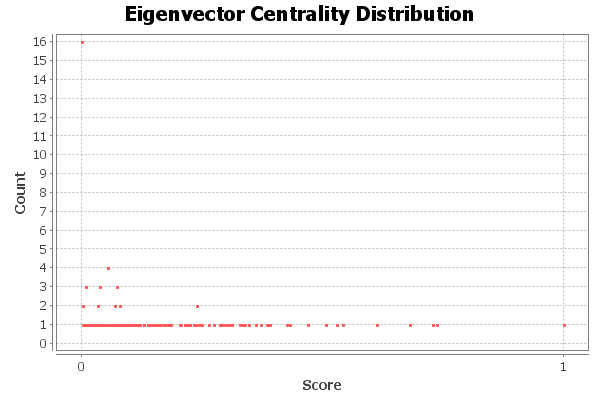
\includegraphics[width=0.5\textwidth,height=\textheight,keepaspectratio]{common_mention_eigenvector_graph.png}}
\caption{Graph for EigenVector Centrality Distribution of Common Mention Network}
\vspace{0.1in}
\centerline{\fontsize{10}{12}{\textbf{Parameters =$>$ Number of iterations: 100, Sum change: 0.007861}}}
\end{figure}

\begin{figure}
\centering
\includegraphics[width=\textwidth,height=\textheight,keepaspectratio]{hashtags_common_network.png}
\caption{Common Hashtags between Celebrities Community Network}
\end{figure}

\begin{figure}
\noindent{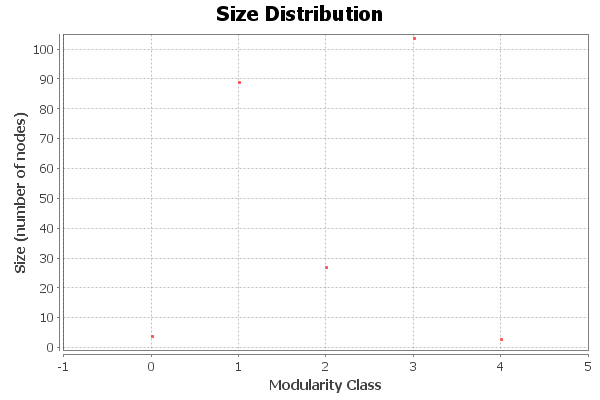
\includegraphics[width=0.45\textwidth,height=\textheight,keepaspectratio]{hashtags_common_modularity_graph.png}}\hspace{1.8cm}{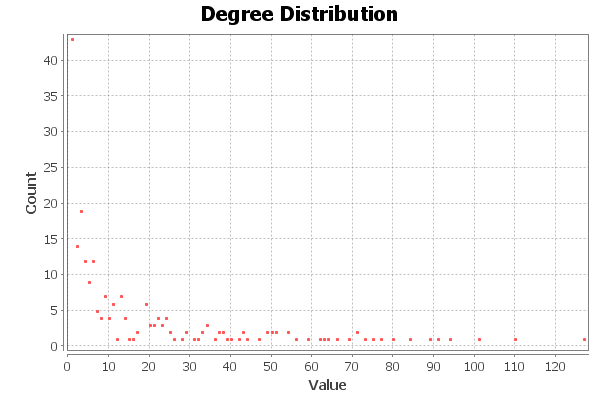
\includegraphics[width=0.45\textwidth,height=\textheight,keepaspectratio]{hashtags_common_degree_graph.png}}
\begin{multicols}{2}{\caption{Graph for the Communities Distribution of Common Hashtags Network}}\vfill\columnbreak{\caption{Graph for the Degree Distribution of Common Hashtags Network}}\end{multicols}
\begin{multicols}{2}{\noindent{\fontsize{10}{12}{\textbf{Results =$>$ Modularity: 0.315, Modularity with resolution: 0.243, Number of Communities: 5}}}}\vfill\columnbreak{\noindent{\fontsize{10}{12}{\textbf{Results =$>$ Average Degree: 18.106}}}}\end{multicols}
\end{figure}

\begin{figure}
\noindent{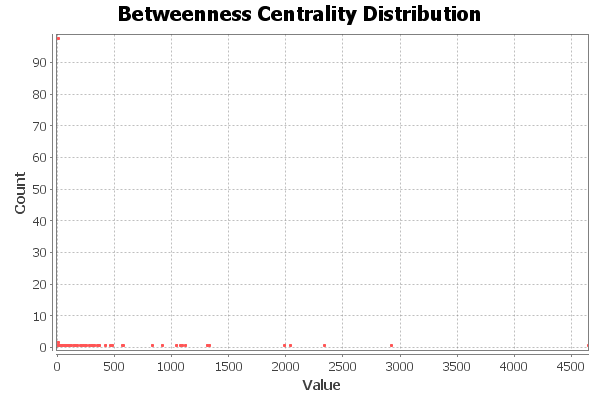
\includegraphics[width=0.45\textwidth,height=\textheight,keepaspectratio]{hashtags_common_betweenness_graph.png}}\hspace{1.8cm}{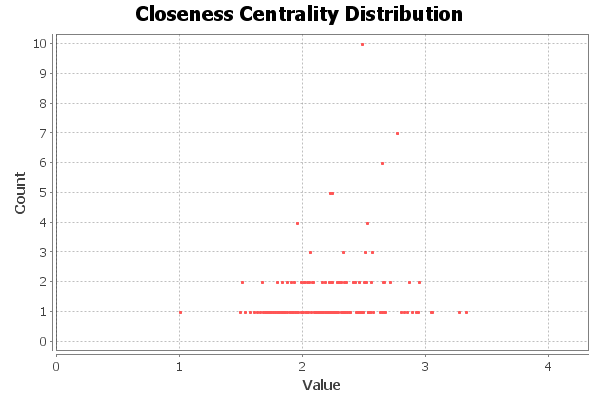
\includegraphics[width=0.45\textwidth,height=\textheight,keepaspectratio]{hashtags_common_closeness_graph.png}}
\begin{multicols}{2}{\caption{Graph for Betweenness Centrality Distribution of Common Hashtags Network}}\vfill\columnbreak{\caption{Graph for Closeness Centrality Distribution of Common Hashtags Network}}\end{multicols}
\end{figure}

\begin{figure}
\centerline{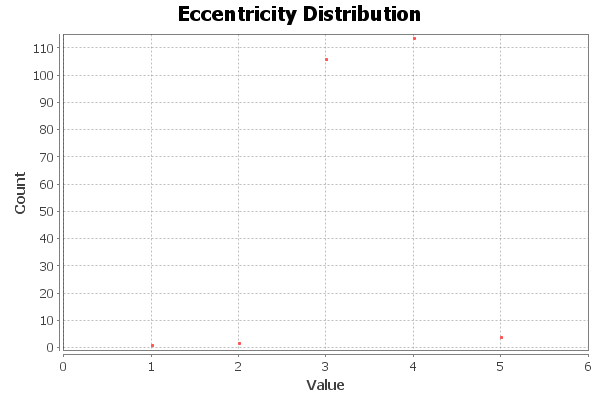
\includegraphics[width=0.50\textwidth,height=\textheight,keepaspectratio]{hashtags_common_eccentricity_graph.png}}
\caption{Graph for Eccentricity Distribution of Hashtags Common Network}
\vspace{0.1in}
\centerline{\fontsize{10}{12}{\textbf{Results =$>$ Diameter: 5, Radius: 1, Average Path length: 2.2723, Number of shortest paths: 49958}}}
\end{figure}

\begin{figure}
\centerline{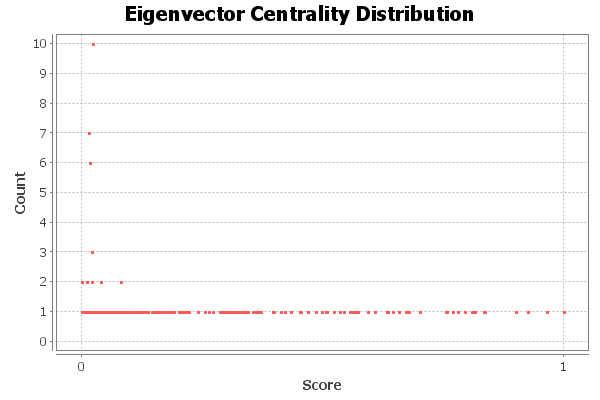
\includegraphics[width=0.5\textwidth,height=\textheight,keepaspectratio]{hashtags_common_eigenvector_graph.png}}
\caption{Graph for EigenVector Centrality Distribution of Common Hashtags Network}
\vspace{0.1in}
\centerline{\fontsize{10}{12}{\textbf{Parameters =$>$ Number of iterations: 100, Sum change: 0.004076}}}
\end{figure}

\section{Conclusion}

\paragraph{}
After analyzing the three networks we get to know about the strength(count) of the users mention for the celebrities and who are the celebrities which tweeters consider most related to each other and to themselves.

\paragraph{}
We also get to know the users who tweet most about celebrities and whether or not they are loyal to one celebrity or many.

\paragraph{}
My study shows that as in accordance to the general perspective the social media also shows the same relationship among the celebrities, making the celebrities from the same community(politics, cinema and cricket) to be related more to each other than with other community and the users being more common between those community celebrities. Surely there are some exceptions but they are overshadowed by the strong relation between the celebrities in single community.

\paragraph{}
For the common users network there were 8 different communities with modularity of 0.351, in this network two clusters were prominent which constitute mostly actors with their related entertainment groups(brown) and politicians with news channels and Government organizations in other(green), the third celebrity group of cricketers were mixed in both these groups and were less in number as compare to other two groups. Surely some communities such as(violet) has some mix of celebrities such as cricketers and actors which has Indian Super League(@IndSuperLeague)(soccer event) as the central group where these celebrities are team owners and other are participating teams twitter handle. Other smaller isolated groups(green,blue) are also connected to each other with their current involvement specific to each other. Within this network two nodes standout due to their size (@narendramodi and @iamsrk) due to their highest betweenness centrality in the two respective clusters within the network which gives us the conclusion that these two celebrities are most commonly mentioned by the users and all other celebrities withn that cluster have users common with these two.

\paragraph{}
For the common mention tweets the network is more spatial and diverse with 17 communities and modularity of 0.580, even here there are two major clusters with same two celebrities(@narendramodi and @iamsrk) having main clout due to their high betweenness centrality, but here due to large number of communities there are some other relevant groups like(violet) of @aamaadmiparty and its members which proposes that these members are more mentioned with each other in a tweet than with others. A single community member(@suhelseth)(violet) strikes out prominently due to his common mention with many other celebrities which is a surprise element in this network. Other isolated communities are also present which is due to their common mention with each other prominently.

\paragraph{}
The third network on the common hashtags between celebrities has 5 communities with modularity 0.315, is more concentrated and could be easily seen to be divided in three major clusters. This network is vastly different from the other two networks as here the three main celebrities due to their betweenness centrality are(@ibnlive, @deepikapadukone and @sonamkapoor) which is different from the previous one's and are quite surprising which holds out that these celebrities are mostly mentioned with the hashtags concerning with other celebrities as well as most are connected to them. Here a third community(red) is also prominent cluster which contains more of sport celebrities connected with each other due to Indian Super League(@IndSuperLeague) event with stark inclusion of some actors which are not part of that event which makes us believe that these celebrities when mentioned are affiliated with these hashtags.

\paragraph{}
Some celebrities or organizations have a very large number of mentions than others which may be due to those celebrities(politicians, cricketers and movie stars) being trending in India for some cause (movie release, an event being taking place or due to their certain initiatives) examples of which could be given with @iamsrk, @deepikapadukone movie stars mentioned a lot due to their movie released within this time period or @IndSupLeague an organization which is conducting a football event within India during this time or @narendramodi India Prime Minister for starting a cleanliness drive campaign within the country.

\paragraph{}
The common mention between some celebrities also has some great numbers like for @iamsrk, @deepikapadukone, @juniorbachchan, @farahkhan are mentioned a great number of times with each other due to a movie release which had all of them working together. The same was for the teams like @FCGoa, @atlidkolkata, @PuneFC and others due to their involvement in a league.

\paragraph{}
Taking all three networks in consideration finally I could say that one celebrity which stands out in the whole network as a whole would be(@narendramodi) India's Prime Minister as he has been the most prominent player in all three networks which comes out as a great signal for the India country as a whole as most of the celebrities and tweeting community could relate to the supreme power of the country which should bring Governance to a smooth start and portends bright future for this country prospects as people are more united and related with the works of Government.

\paragraph{}
Finally I could say that if popularity could be gauged by the mention of celebrities it would hold true to what general perspective is. Still as a caveat before considering this study as the real truth among celebrities relationship is that the study is solely based on the social media mention of celebrities and has been done for a short period of time if the research could be extended to a different level it could be validated to some extent with the real world.

\begin{thebibliography}{3}

\bibitem{1} \href{http://nwb.cns.iu.edu/papers/2007-herr-movieact.pdf}Movies and Actors : Mapping the Internet Movie Database - Bruce W. Herr , Katy Borner
\vspace{0.1in}
\bibitem{2} \href{http://www.mpi-sws.org/~mmarcon/SocialNetworks-IMC.pdf}Measurement and Analysis of Online Social Networks - Alan Mislove, Peter Druschel
\vspace{0.1in}
\bibitem{fafadia} \href{https://github.com/sidharthshah/bollywood-social-network-analysis}Fafadia Tech Blog

\end{thebibliography}

%\href{http://nwb.cns.iu.edu/papers/2007-herr-movieact.pdf}
%\href{http://www.mpi-sws.org/~mmarcon/SocialNetworks-IMC.pdf}
%\href{https://github.com/sidharthshah/bollywood-social-network-analysis}

\end{document}
